\section{Measurement Platforms} \label{sec:measurement-platforms}

The following chapter describes the measurement platforms that were used to
measure and collect data.

\subsection{RIPE Atlas} \label{sec:ripe-atlas}

RIPE~Atlas is an open measurement platform to perform basic measurements on the
internet. It holds more than ten thousand probes that serve as start points. A
probe is machine that has the RIPE Atlas probe software installed. A user can
request a probe for a measurement (e.g., a ping from a probe to a RIPE NCC root
server).

RIPE Atlas offers the following basic types of measurements:

\begin{itemize}
	\item Ping
	\item Traceroute
	\item (Dis)connection Events
	\item DNS Lookup
	\item DNS TLDs
	\item HTTP
	\item TLS (SSL) GET Certificate
\end{itemize}

\begin{wraptable}{r}{7cm}
	\caption{Number of Probes per Country with ASN 14593 on RIPE Atlas}
	\label{fig:probes-per-country}
	\begin{tabular}{lr}
		\toprule
		Country                     & Count \\
		\midrule
		Falkland Islands (Malvinas) & 1     \\
		Réunion                     & 1     \\
		Kiribati                    & 2     \\
		Canada                      & 13    \\
		Poland                      & 1     \\
		Haiti                       & 3     \\
		Spain                       & 4     \\
		Czechia                     & 1     \\
		United States               & 55    \\
		France                      & 18    \\
		Italy                       & 3     \\
		United Kingdom              & 10    \\
		Guam                        & 1     \\
		Australia                   & 9     \\
		Chile                       & 1     \\
		Netherlands                 & 2     \\
		Sweden                      & 2     \\
		Greece                      & 1     \\
		Austria                     & 3     \\
		Belgium                     & 2     \\
		Switzerland                 & 1     \\
		Philippines                 & 3     \\
		Benin                       & 2     \\
		Virgin Islands, U.S.        & 1     \\
		Germany                     & 9     \\
		Madagascar                  & 1     \\
		\bottomrule
	\end{tabular}
\end{wraptable}

RIPE Atlas offers the possibility to start measurements via the web interface
or an API. While the web interface is sufficient for most use cases, it is also
quite limited. Using the API offers more possibilities (e.g., turning DoH
queries into DoTLS by adding \verb|"tls": true| into the definition of the
measurement).

Additionally, each registered probe performs measurements on a regular basis in
fixed time intervals (e.g., each probe performs every 240 seconds a ping
measurement against all RIPE NCC root servers). Those measurements are called
built-in measurements. They run always when the probe is only and connected to
the RIPE Atlas network. The built-in measurements are the ones used for the
data of this thesis within a specified time interval (usually January 2022 to
June 2024).

Downloading the results of a measurement also works by accessing the API. For
previous results, one can access the REST API that stores all results ever
measured. For more up-to-date results, one can use the Streaming API that sends
the most recent results to a subscribed socket. Theoretically, the API is
rate-limited, but we did not encounter problems even when bulk-downloading
larger datasets. Still, ethical crawling was used.

RIPE Atlas offered 150 Starlink probes (i.e., probes with ASN14593) at the time
of writing. Table~\ref{fig:probes-per-country} shows the number of probes per
country. The originating country is determined by RIPE Atlas.
\subsection{Cloudflare Radar} \label{sec:cloudflare-radar}

Cloudflare manages a vast amount of traffic on the internet. Initially, it
served the purpose of protecting servers from attacks. Today amongst others, it
also manages traffic, and sells data. In 2020, Cloudflare released data that
has been held internal. This new platform is \ac{CFR}. \ac{CFR} offers various
statistics on the internet ranging from security statistics over latency
measurements to bot ratios per country.

For the purpose of this thesis, we are mostly interested in the performance
measurements. \ac{CFR} offers performance measurements within their \ac{IQI}.
It is the collection of measurements performed through their
\href{https://speed.cloudflare.com/}{Internet Speed Test}
\cite{DavidBelson2023, CloudflareRadarDocsIQI}. As target, \ac{CFR} uses a
fixed set of Cloudflare servers.

\begin{takeaway}{Difference of RIPE Atlas and Cloudflare Radar}
	Measurements performed in \ac{CFR} and RIPE Atlas differentiate in the
	targeted servers (root servers vs. Cloudflare servers), the measurement
	probe (RIPE Atlas probe vs. browser), and the metric used (TLS vs. Time
	to First Byte). Cloudflare's servers are expected to have a better
	latency (they claim to be ~50ms away from 95 \% of the earth's
	population; State September 17, 2024).
\end{takeaway}

\begin{figure}
	\begin{subfigure}[t]{0.48\textwidth}
		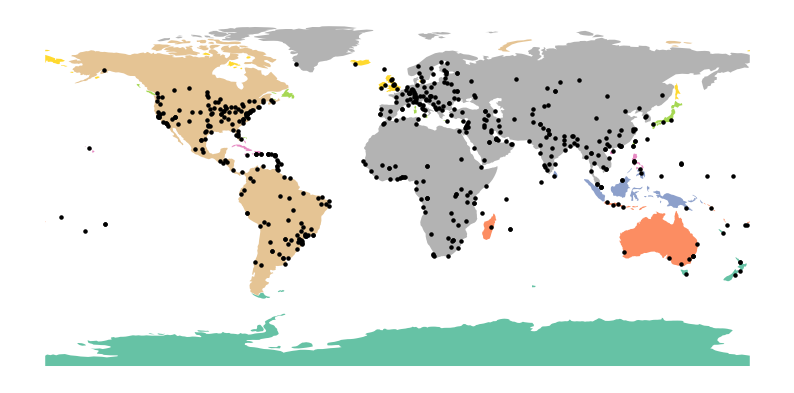
\includegraphics[width=\textwidth]{./chapters/3-methodology/img/rootserver-locations.png}
		\caption{Locations of Root Servers (all *.root-servers.org
			together) \cite{rootservers092024}}
	\end{subfigure}
	\begin{subfigure}[t]{0.48\textwidth}
		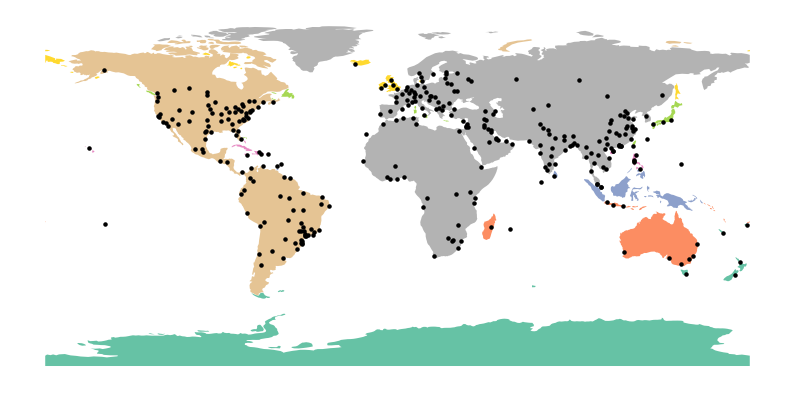
\includegraphics[width=\textwidth]{./chapters/3-methodology/img/cloudflare-datacenter-locations.png}
		\caption{Locations of Cloudflare Data Centers
			\cite{CloudflareGlobalNetwork2024}}
	\end{subfigure}
\end{figure}

% TODO: Do I actually need this?
\subsection{OONI} \label{sec:ooni}

\subsection{N2YO} \label{sec:n2yo}

N2YO is a platform collecting data about satellites in space. It is a data
integration platform collecting data from different platforms like Celestrak
and Space-Track.

For the purpose of this thesis, N2YO is used to find information on the
development of various satellite constellations. Therefore, we want to find the
following information:

\begin{itemize}
	\item Satellite ID (also formerly called Norad ID)
	\item Satellite Name
	\item Launch Date
	\item Decay Date (if applicable)
	\item Classification (if applicable)
\end{itemize}

Each satellite receives a unique ID, centrally given to all satellites
launched. It is a continuous number starting at 1. The satellite with ID~1 is
the rocket body of Sputnik~1. Sputnik~1 itself holds ID~2.

The data is obtained by a web crawler that parses the HTML page and finds the
information needed. There is also the possibility of getting the data by API,
but the API is rate-limited. Parsing HTML is inefficient, but still a quicker
approach compared to using the API.
